%% This is file `elsarticle-template-1-num.tex',
%%
%% Copyright 2009 Elsevier Ltd
%%
%% This file is part of the 'Elsarticle Bundle'.
%% ---------------------------------------------
%%
%% It may be distributed under the conditions of the LaTeX Project Public
%% License, either version 1.2 of this license or (at your option) any
%% later version.  The latest version of this license is in
%%    http://www.latex-project.org/lppl.txt
%% and version 1.2 or later is part of all distributions of LaTeX
%% version 1999/12/01 or later.
%%
%% Template article for Elsevier's document class `elsarticle'
%% with numbered style bibliographic references
%%
%% $Id: elsarticle-template-1-num.tex 149 2009-10-08 05:01:15Z rishi $
%% $URL: http://lenova.river-valley.com/svn/elsbst/trunk/elsarticle-template-1-num.tex $
%%
\documentclass[preprint,12pt]{elsarticle}

%% Use the option review to obtain double line spacing
%% \documentclass[preprint,review,12pt]{elsarticle}

%% Use the options 1p,twocolumn; 3p; 3p,twocolumn; 5p; or 5p,twocolumn
%% for a journal layout:
%% \documentclass[final,1p,times]{elsarticle}
%% \documentclass[final,1p,times,twocolumn]{elsarticle}
%% \documentclass[final,3p,times]{elsarticle}
%% \documentclass[final,3p,times,twocolumn]{elsarticle}
%% \documentclass[final,5p,times]{elsarticle}
%% \documentclass[final,5p,times,twocolumn]{elsarticle}

%% The graphicx package provides the includegraphics command.
\usepackage{graphicx}
%% The amssymb package provides various useful mathematical symbols
\usepackage{amssymb}

\usepackage{amsmath} % assumes amsmath package installed
\usepackage{amssymb}  % assumes amsmath package installed
\usepackage{mathrsfs}
\usepackage{bbm}
\usepackage{float}
\usepackage{tikz}
\usepackage[spanish]{babel}
\selectlanguage{spanish}
\usepackage[utf8]{inputenc}
\usepackage{algorithm}
\usepackage[colorinlistoftodos]{todonotes}
\usepackage[colorlinks=true, allcolors=blue]{hyperref}
\usepackage[noend]{algorithmic}

\newenvironment{theorem}[2][Theorem]{\begin{trivlist}
\item[\hskip \labelsep {\bfseries #1}\hskip \labelsep {\bfseries #2.}]}{\end{trivlist}}
\newenvironment{lemma}[2][Lemma]{\begin{trivlist}
\item[\hskip \labelsep {\bfseries #1}\hskip \labelsep {\bfseries #2.}]}{\end{trivlist}}
\newenvironment{exercise}[2][Exercise]{\begin{trivlist}
\item[\hskip \labelsep {\bfseries #1}\hskip \labelsep {\bfseries #2.}]}{\end{trivlist}}
\newenvironment{problem}[2][Problem]{\begin{trivlist}
\item[\hskip \labelsep {\bfseries #1}\hskip \labelsep {\bfseries #2.}]}{\end{trivlist}}
\newenvironment{question}[2][Question]{\begin{trivlist}
\item[\hskip \labelsep {\bfseries #1}\hskip \labelsep {\bfseries #2.}]}{\end{trivlist}}
\newenvironment{corollary}[2][Corollary]{\begin{trivlist}
\item[\hskip \labelsep {\bfseries #1}\hskip \labelsep {\bfseries #2.}]}{\end{trivlist}}

\newenvironment{solution}{\begin{proof}[Solution]}{\end{proof}}
 
    
%% The amsthm package provides extended theorem environments
%% \usepackage{amsthm}

%% The lineno packages adds line numbers. Start line numbering with
%% \begin{linenumbers}, end it with \end{linenumbers}. Or switch it on
%% for the whole article with \linenumbers after \end{frontmatter}.
\usepackage{lineno}

%% natbib.sty is loaded by default. However, natbib options can be
%% provided with \biboptions{...} command. Following options are
%% valid:

%%   round  -  round parentheses are used (default)
%%   square -  square brackets are used   [option]
%%   curly  -  curly braces are used      {option}
%%   angle  -  angle brackets are used    <option>
%%   semicolon  -  multiple citations separated by semi-colon
%%   colon  - same as semicolon, an earlier confusion
%%   comma  -  separated by comma
%%   numbers-  selects numerical citations
%%   super  -  numerical citations as superscripts
%%   sort   -  sorts multiple citations according to order in ref. list
%%   sort&compress   -  like sort, but also compresses numerical citations
%%   compress - compresses without sorting
%%
%% \biboptions{comma,round}

% \biboptions{}

\journal{Journal Name}

\begin{document}

\begin{frontmatter}

%% Title, authors and addresses

\title{Cómputo Científico \\ Tarea VIII}

%% use the tnoteref command within \title for footnotes;
%% use the tnotetext command for the associated footnote;
%% use the fnref command within \author or \address for footnotes;
%% use the fntext command for the associated footnote;
%% use the corref command within \author for corresponding author footnotes;
%% use the cortext command for the associated footnote;
%% use the ead command for the email address,
%% and the form \ead[url] for the home page:
%%
%% \title{Title\tnoteref{label1}}
%% \tnotetext[label1]{}
%% \author{Name\corref{cor1}\fnref{label2}}
%% \ead{email address}
%% \ead[url]{home page}
%% \fntext[label2]{}
%% \cortext[cor1]{}
%% \address{Address\fnref{label3}}
%% \fntext[label3]{}


%% use optional labels to link authors explicitly to addresses:
%% \author[label1,label2]{<author name>}
%% \address[label1]{<address>}
%% \address[label2]{<address>}

\author{Joel Chac\'on Castillo}

\address{Guanajuato, M\'exico}
\end{frontmatter}



\section{Simulación Normal bivariada}
Aplique el algoritmo de Metropolis-Hastings considerando como función objetivo la distribuición normal bivariada:
\begin{equation}
    f_{x_1, x_2}(x) = \frac{1}{2 \pi} | \Sigma |^{\frac{-1}{2}} exp \{ -\frac{1}{2} (x-\mu)^T \Sigma^{-1} (x-\mu) \}
\end{equation}
donde 
\begin{equation}
    \mu = \begin{pmatrix} \mu_1 \\ \mu_2 \end{pmatrix}
    \Sigma = \begin{pmatrix} \sigma_1^2 & \rho \sigma_1 \sigma_2 \\ \rho \sigma_1 \sigma_2 & \sigma_2^2 \end{pmatrix}
\end{equation}
Donde se tienen las siguientes distribución condicionales:
\begin{equation}
    \begin{split}
        X_1 | X_2 &= x_2 \sim N \left (\mu_1 + \rho \frac{\sigma_1}{\sigma_2} (x_2 - \mu_2), \sigma_1^2 (1-\rho^2)  \right ) \\
        X_2 | X_1 &= x_1 \sim N \left (\mu_2 + \rho \frac{\sigma_2}{\sigma_1} (x_1 - \mu_1), \sigma_2^2 (1-\rho^2)  \right )
    \end{split}
\end{equation}
considere las siguientes propuestas:
\begin{equation}
    \begin{split}
        q_1 (( x_1 \prime , x_2 \prime) | (x_1, x_2)) = f_{X_1 | X_2} (x_1 \prime | x_2 ) \mathbbm{1}(x_2 \prime = x_2) \\
        q_2 (( x_1 \prime , x_2 \prime) | (x_2, x_1)) = f_{X_2 | X_1} (x_2 \prime | x_1 ) \mathbbm{1}(x_1 \prime = x_1)
    \end{split}
\end{equation}
A partir del algoritmo MH usando Kernels híbridos simule valores de la distribución normal bivariada, fijando $\sigma_1 = \sigma_2 = 1$, considere los casos donde $\rho = 0.8$ y $\rho=0.99$.

\subsection*{Comentarios}

Primero se establece una relación entre el método de Metrópolis Hastings y el método de muestreo de Gibbs mencionado en la pag. 381 de \cite{robert2010introducing} (esto también se vió en clase).

\begin{theorem} 1
EL método de muestreo de Gibbs es equivalente a la composición de P-algoritmos  de Metrópolis Hastings, con probabilidad de aceptación uniformemente igual a la unidad.
\end{theorem}
 
En consecuencia nunca se rechaza el criterio de aceptación para este caso,

La implementación está basada en el \textit{Random Scan Gibbs Sampler} donde cada kernel se selecciona con probabilidad $\omega$, como se indica en al siguiente ecuación:
\begin{equation}
\begin{split}
    K &= \sum_{i=0}^n \omega_i k_i \\
    s.a. & \quad \sum_i \omega_i = 1
\end{split}
\end{equation}
Se aclara que en el código no se aplica el kernel cero para forzar que la cadena sea fuértemente aperiódica.
%



\section{Simulación distribución Weibull}
Considere los tiempos de falla $t_1, ..., t_n$ con distribución de Weibull($\alpha, \lambda$):
\begin{equation}
    f(t_i | \alpga, \lambda) = \alpha \lambda t_i^{\alpha-1} e^{-t_i^\alpha \lambda}
\end{equation}
Se asumen como a priori $\alpha \sim exp(c)$ y $\lambda | \alpha \sim Gamma(a, b)$, por lo tanto, $f(\alpha, \lambda) = f(\lambda | \alpha) f(\alpha)$.
%
Así, para la distribución posterior se tiene:
\begin{equation}
    f(\alpha, \lambda | \hat{t}) \propto f(\hat{t} | \alpha, \lambda) f(\alpha, \lambda)
\end{equation}
A partir del algoritmo MH usando Kernels híbridos simule valores de la distribución posteriori $f(\alpha, \lambda | \hat{t})$, considerando las siguiente propuestas:

\begin{itemize}
    \item Propuesta 1: 
    \begin{equation}
    \lambda_p| \alpha,\hat{t} \sim Gamma( \alpha +b, b + \sum_{i=1}^n t_i^\alpha)  
    \end{equation}
    dejando $\alpha$ fijo.
    \item Propuesta 2:
    \begin{equation}
        \alpha_p | \lambda, \hat{t} \sim Gamma(n+1, -log(b) - log(r_1) + c)
    \end{equation}
    con $r_i = \prod_{i=1}^n t_i$, dejando $\lambda$ fijo.
    \item Propuesta 3:
    \begin{equation}
        \alpha_p \sim exp(c) \\
        \lambda_p | \alpha_p \sim Gamma(\alpha_p, b)
    \end{equation}
    \item Propuesta 4 (RWMH):
    $\alpha_p = \alpha + \epsilon$ con $\epsilon \sim N(0, \sigma)$ y dejando $\lambda$ fijo.
\end{itemize}
Simular datos utilizando $\alpha=1$ y $\lambda=1$ con $n=20$. Para la a priori utilizar $c=1$ y $b=1$.

\subsection*{Comentarios}

\section{Problema de las bombas de agua en la central nuclear}
Considere el ejemplo referente al número de fallas de bombas de agua en una central nuclear \cite{robert2010introducing} \cite{norton2018sampling}, donde $p_i$ representa el número de falls en el tiempo de operación $t_i$, con $i=1, ..., n$.
%
Se considera el modelo $p_i \sim Poisson(\lambda_i t_i)$, (las $\lambda_i$ son independientes entre si), con distribuciones a priori $\lambda_i | \beta \sim Gamma(\alpha, \beta)$ y $\beta \sim Gamma(\gamma, \delta)$, por lo tanto:
\begin{equation}
    f(\lambda_1, ..., \lambda_n, \beta) = f(\lambda_1 | \beta)....f(\lambda_n | \beta) f(\beta)
\end{equation}
Para la distribución posterior se tiene
\begin{equation}
    f(\lambda_1, ..., \lambda_n, \beta | \hat{p}) \propto L(\hat{p}, \hat{\lambda}, \beta) f(\lambda_1,...,\lambda_n , \beta) 
\end{equation}
Simule valores de la distribución posterior $f(\lambda_1, ..., \lmabda_n, \beta | \hat{p})$ usando un kernel híbrido, considerando las propuestas:
\begin{itemize}
    \item $\lambda_1 | \hat{\lambda_i}, \beta, \hat{y} \sim Gamma(p_i + \alpha, t_i + \beta)$
    \item $\beta | \hat{\lambda}, \hat{t} \sim Gamma( n \alpha + \gamma, \delta + \sum_{i=1}^n \lambda_i  )$
\end{itemize}
verifique que estas son propuestas de Gibbs. Utilizar la siguiente tabla con los parámetros a priori $\alpha=1.8$, $\gamma = 0.01$ y $\delta=1$.

\begin{table}[H]
\begin{tabular}{|c|c|c|c|c|c|c|c|c|c|c|}
\hline
\textbf{Pump}     & 1     & 2     & 3     & 4      & 5    & 6     & 7    & 8    & 9    & 10    \\ \hline
\textbf{Failures} & 5     & 1     & 5     & 14     & 3    & 19    & 1    & 1    & 4    & 22    \\ \hline
\textbf{Time}     & 94.32 & 15.72 & 62.88 & 125.76 & 5.24 & 31.44 & 1.05 & 1.05 & 2.10 & 10.48 \\ \hline
\end{tabular}
\end{table}

\subsection*{Comentarios}
Dada las distribuciones a priori asociadas $\lambda_i \sim Gamma(\alpha, \beta)$, $\beta \sim Gamma(\gamma, \delta)$.
%
La distribución conjunta es entonces:
\begin{equation}
    \begin{split}
    &\pi(\lambda_1, ..., \lambda_{10}, \beta | t_1, ..., t_{10}, p_1, .., p_{10}) \\  &\propto    \prod_{i=1}^{10} \{ (\lambda_i t_i)^{p_i} e^{-\lambda_i t_i} \lambda_i^{\alpha-1} e^{-\beta \lambda_i} \} \beta^{10 \alpha} \beta^{\gamma-1} e^{-\delta \beta} \\
       & \propto \prod_{i=1}^{10} \{ \lambda_i^{p_i + \alpha -1} e^{-(t_i + \beta)\lambda_i} \} \beta^{10 \alpha + \gamma -1} e^{-\delta \beta}
    \end{split}
\end{equation}
y siguiendo una descomposición natural (esta descomposición refleja la estructura jeráquica del modelo) de $\pi$ en las distribucionles condicionales se tiene lo siguiente:

\begin{equation}
    \begin{split}
          \lambda_1 | \hat{\lambda_i}, \beta, \hat{y} \sim Gamma(p_i + \alpha, t_i + \beta) \\
     \beta | \hat{\lambda}, \hat{t} \sim Gamma( n \alpha + \gamma, \delta + \sum_{i=1}^n \lambda_i  )
    \end{split}
\end{equation}

Por lo tanto queda verificado que estas propuestas son Gibbs, pues muestreando de las distribuciones condicionales es posible simular la distribución posteriori.



Esta simulación se programó considerando un burn-in de 1000 iteraciones y un número total de iteraciones de 10000.
%
En la siguiente tabla se muestra el promedio obtenido de los estados visitados por la cadena de markov (sin considerar el burn-in).
%
Se menciona que los tanto la tabla como las propuestas están distintas en el libro \cite{robert2010introducing} de que en las instrucciones de la tarea.
%
% Please add the following required packages to your document preamble:
% \usepackage{graphicx}
\begin{table}[]
\resizebox{\textwidth}{!}{%
\begin{tabular}{c|c|c|c|c|c|c|c|c|c|c|c|}
\cline{2-12}
\textbf{}                                              & $\beta$ & $\lambda_1$ & $\lambda_2$ & $\lambda_3$ & $\lambda_4$ & $\lambda_5$ & $\lambda_6$ & $\lambda_7$ & $\lambda_8$ & $\lambda_9$ & $\lambda_10$ \\ \hline
\multicolumn{1}{|c|}{\textbf{Resultados obtenido}}     & 2.712   & 0.067       & 0.1545      & 0.0968      & 0.1200      & 0.6746      & 0.6174      & 0.8774      & 0.9140      & 1.2795      & 1.8028       \\ \hline
\multicolumn{1}{|c|}{\textbf{Resultados  de la tesis}} & -       & 0.059       & 0.102       & 0.089       & 0.116       & 0.116       & 0.609       & 0.893       & 0.881       & 1.584       & 1.992        \\ \hline
\end{tabular}%
}
\end{table}

Los resultados obtenidos fueron los mismos que se mencionan en el trabajo de \cite{norton2018sampling}, es decir $\beta = 2.5$

\begin{figure}[H]
\centering
\begin{tabular}{c c}
\includegraphics[scale=0.3]{Images/pdf_Beta_Hasting_r2.eps}      &\includegraphics[scale=0.3]{Images/pdf_Truncated_Normal_Hasting_r2.eps}   \\
\includegraphics[scale=0.3]{Images/pdf_Uniform_Hasting_r2.eps}      &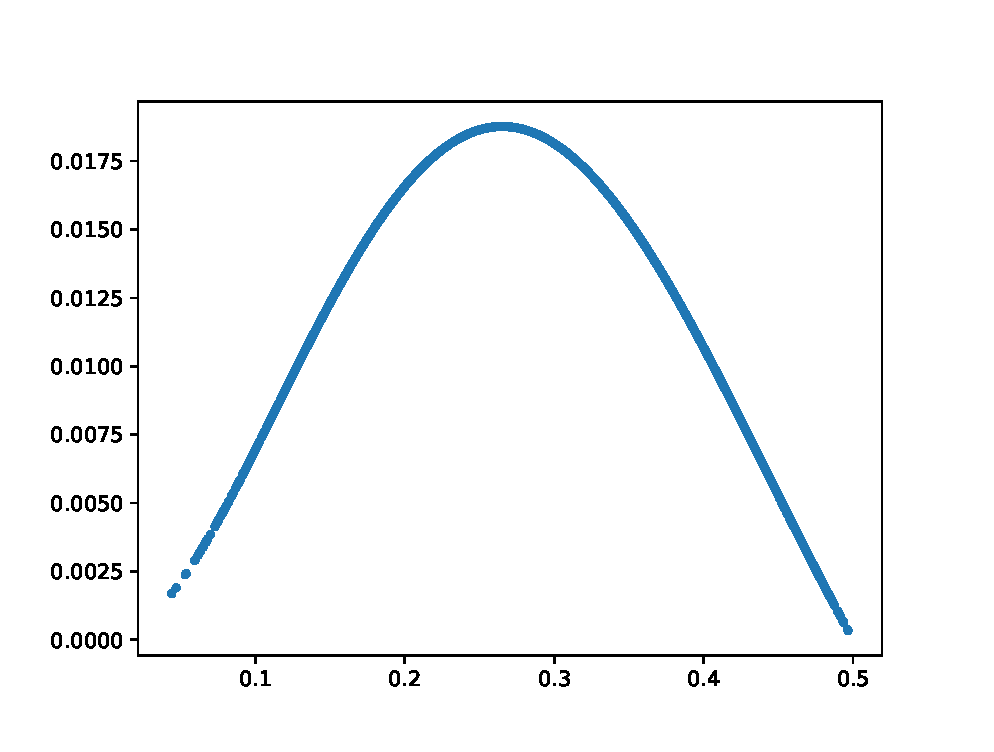
\includegraphics[scale=0.3]{Images/Real_pdf_r2.eps}  
\end{tabular}
\caption{PDF de de tres distribuciones instrumentales, beta, uniforme y normal truncada. En la parte inferior derecha el pdf de la función posteriori a simular considerando n=5. Se consideraron 10'000 iteraciones.} \label{fig2}.
\end{figure}


%%
%% Start line numbering here if you want
%%
\linenumbers

%% main text

%% The Appendices part is started with the command \appendix;
%% appendix sections are then done as normal sections
%% \appendix

%% \section{}
%% \label{}

%% References
%%
%% Following citation commands can be used in the body text:
%% Usage of \cite is as follows:
%%   \cite{key}          ==>>  [#]
%%   \cite[chap. 2]{key} ==>>  [#, chap. 2]
%%   \citet{key}         ==>>  Author [#]

%% References with bibTeX database:

\bibliographystyle{model1-num-names}
\bibliography{sample.bib}

%% Authors are advised to submit their bibtex database files. They are
%% requested to list a bibtex style file in the manuscript if they do
%% not want to use model1-num-names.bst.

%% References without bibTeX database:

% \begin{thebibliography}{00}

%% \bibitem must have the following form:
%%   \bibitem{key}...
%%

% \bibitem{}

% \end{thebibliography}


\end{document}

%%
%% End of file `elsarticle-template-1-num.tex'.